\documentclass{beamer}
%% Possible paper sizes: a0, a0b, a1, a2, a3, a4.
%% Possible orientations: portrait, landscape
%% Font sizes can be changed using the scale option.
\usepackage[size=a3,orientation=portrait,scale=1.8]{beamerposter}
\usetheme{LLT-poster}
\usecolortheme{ComingClean}
% \usecolortheme{Entrepreneur}
% \usecolortheme{ConspiciousCreep}  %% VERY garish.

\usepackage[utf8]{inputenc}
\usepackage[spanish]{babel}
\usepackage[T1]{fontenc}
\usepackage{libertine}
\usepackage[scaled=0.92]{inconsolata}
\usepackage[libertine]{newtxmath}
\usepackage[numbers]{natbib}
\renewcommand{\bibfont}{\small}

\newcommand{\texthash}{\#}


%% Load the markdown package
\usepackage[citations,footnotes,definitionLists,hashEnumerators,smartEllipses,tightLists=false,pipeTables,tableCaptions,hybrid]{markdown}
%%begin novalidate
\markdownSetup{rendererPrototypes={
 link = {\href{#2}{#1}},
 headingFour = {\begin{block}{#1}},
 horizontalRule = {\end{block}}
}}
%%end novalidate

\author[fis.carlosmanuel@gmail.com]{Carlos Manuel Rodríguez Martínez}
\title{Simulación de bolsa de valores usando Jason/CArtAgO}
\institute{Universidad Veracruzana}
% Optional foot image
\footimage{
\includegraphics[width=4cm]{yop.jpeg}}

\begin{document}
\begin{frame}[fragile]\centering

\begin{columns}
\begin{column}{0.57\textwidth}

\begin{markdown}

#### Resúmen
Se realizo la ejecución de una simulación de una subasta doble que representa una bolsa de valores en la cual operan dos tipos de agentes:

* Agentes con Zero Inteligencia (ZI): Son agentes que realizan operaciones de compra/venta dependiendo de variables aleatorias generadas por distribuciones de probabilidad.
* Agentes Media Móvil (MA): Son agentes que deciden si comprar o vender dependiendo de la cruza de medias móviles.

----
\end{markdown}
\end{column}

\begin{column}{.4\textwidth}
\begin{markdown}

#### Características añadidas

* Ambiente híbrido que soporta CArtAgO y TimeSteppedEnviroment.
* Implementación de estrategia Moving Average.
* Implementación de agente con estrategia definida en Wolfram Language.
* Inicialización de parámetros por medio de artefacto CArtAgO con interfaz gráfica.
* Generación de Log de libro de órdenes.


----
\end{markdown}
\end{column}

\end{columns}

\bigskip
{\usebeamercolor[bg]{headline}\hrulefill}
\bigskip

\begin{columns}[T]

%%%% First Column
\begin{column}{.46\textwidth}

\begin{markdown}

#### Arquitectura

\begin{figure}[h!]
\centering
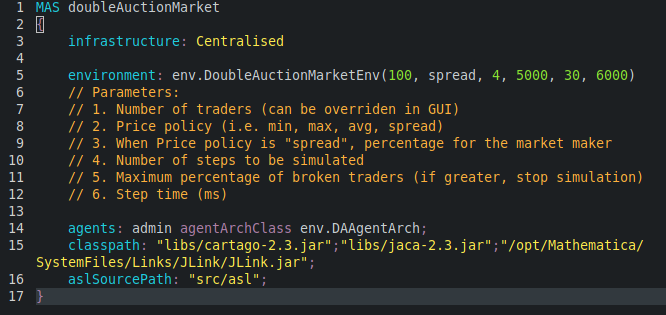
\includegraphics[scale=0.3]{img/code.png}
\end{figure}

* La simulación se realiza en un ambiente llamado *DoubleAuctionMarketEnv*.
* Este ambiente comienza levantando CArtAgO, y genera un artefacto GUI que recibe parámetros del usuario (ambiente externo).
* En cuanto el artefacto envía la señal de comenzar, el administrador crea a los traders, envía parámetros, y finaliza terminando su existencia y cerrando los servicios CArtAgO.
* Comienza la simulación en el ambiente usando *acciones internas*.

----

#### Simulación de precios

Al evaluar los resultados añadiendo mayor proporción de agentes que siguen la estrategia Moving Average (MA) se observa que el comportamiento de la serie de tiempo de precios adquiere periodicidad hasta llegar a un punto crítico entre 75\% y 80\% de agentes MA en donde la simulación converge a un precio estacionario.

\begin{figure}[h!]
\centering
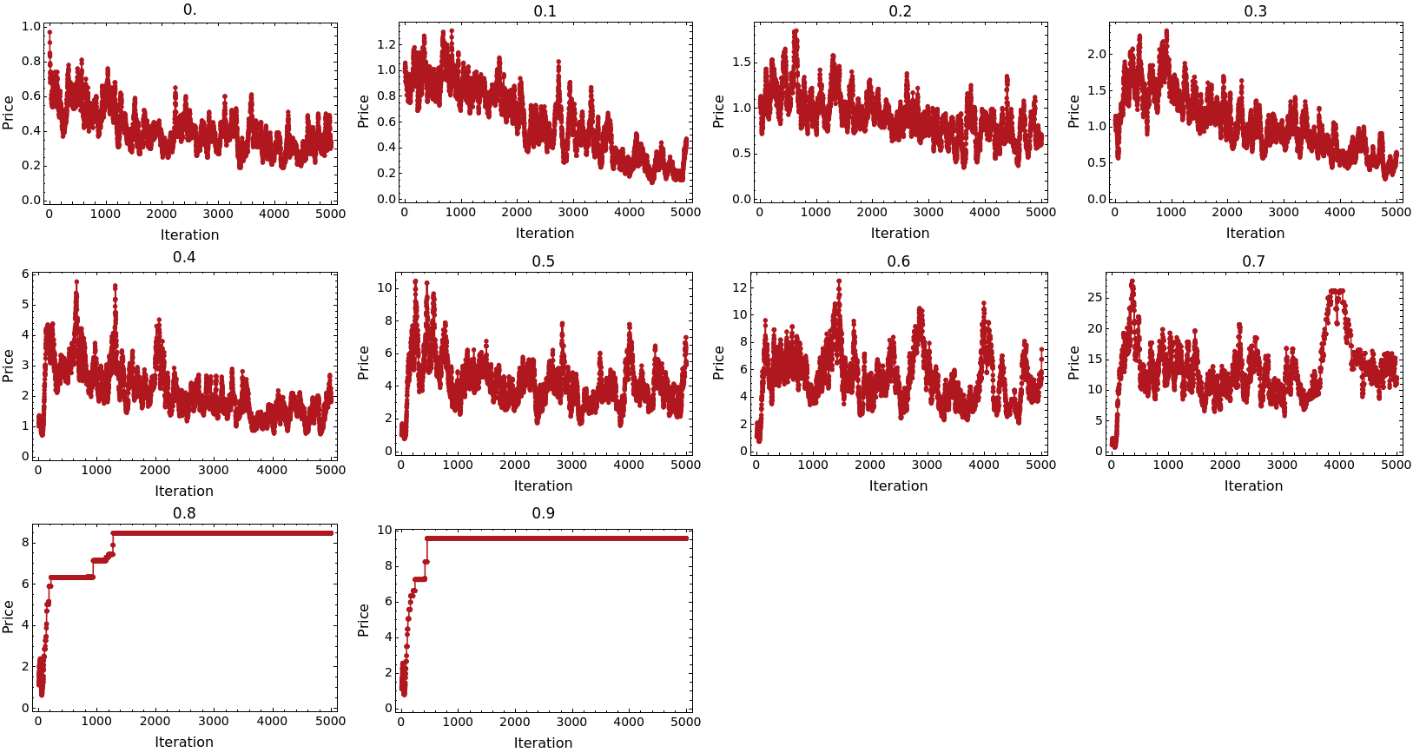
\includegraphics[scale=0.25]{img/price_series.png}
\end{figure}

----

\end{markdown}

\end{column}

%%%% Second Column
\begin{column}{.46\textwidth}

\begin{markdown}

#### Distribuciones de precios

Al comparar con las distribuciones de retornos generadas por la misma serie de precios se observa que al añadir mayor proporción de agentes MA las colas de las distribuciones de retornos se hacen cada vez más pesadas, lo cual es una propiedad deseable de una simulación de un mercado.

\begin{figure}[h!]
\centering
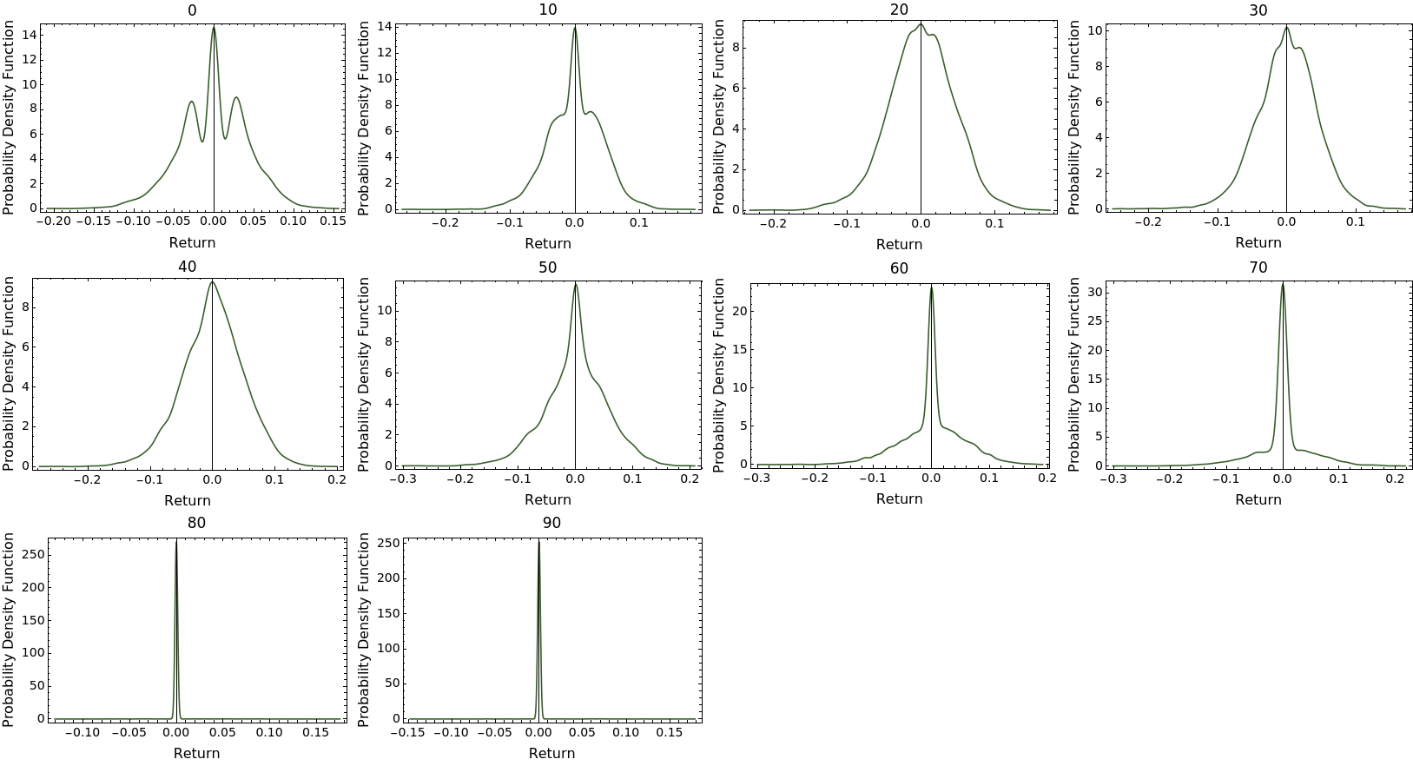
\includegraphics[scale=0.25]{img/dist_prices.png}
\end{figure}

----

#### Comparación de estrategias

Comparando la riqueza promedio de los agentes tipo MA con los ZI es posible concluir que la estrategia MA genera una ventaja significativa con respecto a la estrategia ZI.

\begin{figure}[h!]
\centering
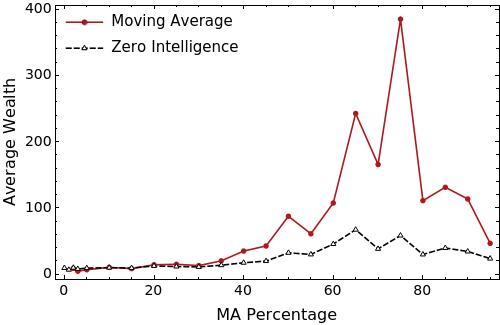
\includegraphics[scale=0.4]{img/wealth_comparison.jpeg}
\end{figure}

----

\end{markdown}
\end{column}
\end{columns}

\end{frame}


\end{document}